% --
% Experiments on whole dataset

\section{Experiments on whole dataset}\label{sec:exp_final}
The final experiments were performed on the whole dataset with 3500 examples per labels and are therefore used for comparison to the benchmark models shown in \rsec{prev_kws_benchmark}.
All Convolutional Neural Network (CNN) architectures were evaluated with 12 MFCC coefficients and the application of frame-based normalization.
A single run with 2000 epochs was performed for all experiments, to save computational effort.
The evaluation on the adversarial pre-training as described in \rsec{exp_adv} was done for the \texttt{conv-jim} model in a separate run.
The results of the experiments are shown in \rtab{exp_final_l12}.
\begin{table}[ht!]
\small
\begin{center}
\caption{Experiment on the whole dataset with 3500 examples per label, 12 MFCC coefficients and 2000 epochs.}
\begin{tabular}{ M{3cm}  M{1.5cm}  M{2.5cm}  M{2.5cm}  M{2.5cm} }
\toprule
\multirow{2}{*}{\centering\textbf{Model Name}} & \multirow{2}{*}{\centering\textbf{Norm.}} & \multirow{2}{*}{\centering\textbf{Pre-Train}} & \multicolumn{2}{c}{\textbf{Accuracy}}\\
& & & Test set & My dataset\\
\midrule
conv-trad & 0 & - & $84.52$ & $92.00$ \\
conv-fstride & 0 & - & $79.76$ & $80.00$ \\
conv-jim & 0 & - & $87.14$ & $88.00$ \\
\midrule
conv-trad & 1 & - & $83.79$ & $88.00$ \\
conv-fstride & 1 & - & $78.71$ & $92.00$ \\
conv-jim & 1 & - & $82.36$ & $88.00$ \\
\midrule
conv-jim & 1 & adv-label-100 & $84.62$ & $92.00$ \\
\bottomrule
\label{tab:exp_final_l12}
\end{tabular}
\end{center}
\vspace{-4mm}
\end{table}
\FloatBarrier
\noindent
Note that there might be some overfitting effects happening, especially showing up in the not normalized training of the \texttt{conv-trad} model in \rtab{exp_final_loss_conv-trad}.
It is therefore useful to use some kind of \emph{early-stopping} technique to obtain the model parameters at the best performing training epoch evaluated on the validation set.
\begin{figure}[!ht]
  \centering
  \subfigure[norm0]{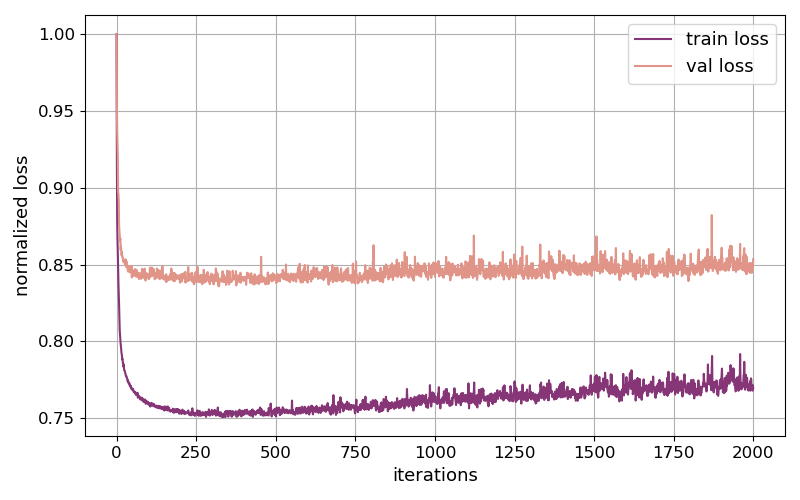
\includegraphics[width=0.45\textwidth]{./5_exp/figs/exp_final_loss_norm0_conv-trad}}
  \subfigure[norm1]{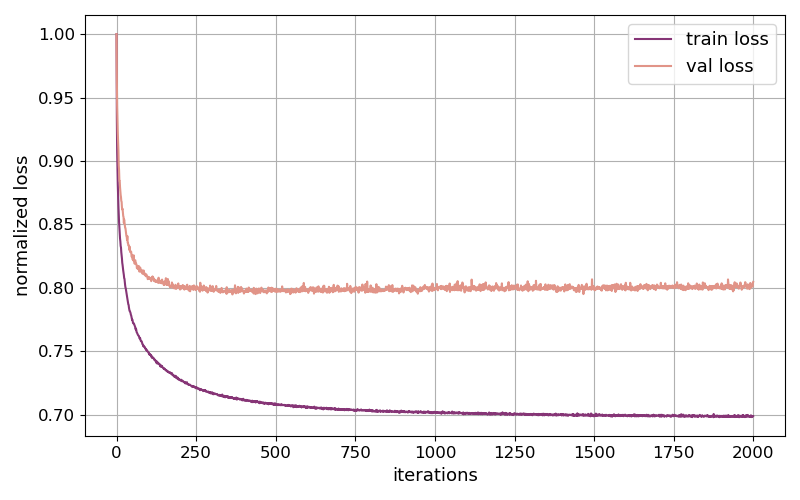
\includegraphics[width=0.45\textwidth]{./5_exp/figs/exp_final_loss_norm1_conv-trad}}
  \caption{Training loss of the \texttt{conv-trad} model showing overfitting effects on the whole dataset.}
  \label{fig:exp_final_loss_conv-trad}
\end{figure}
\FloatBarrier
\noindent
The training of models with frame-based normalization usually has less problems with overfitting compared to when using no normalization.
The accuracy performance on the validation set of all models with and without frame-based normalization is shown in \rtab{exp_final_acc}.
\begin{figure}[!ht]
  \centering
  \subfigure[norm0]{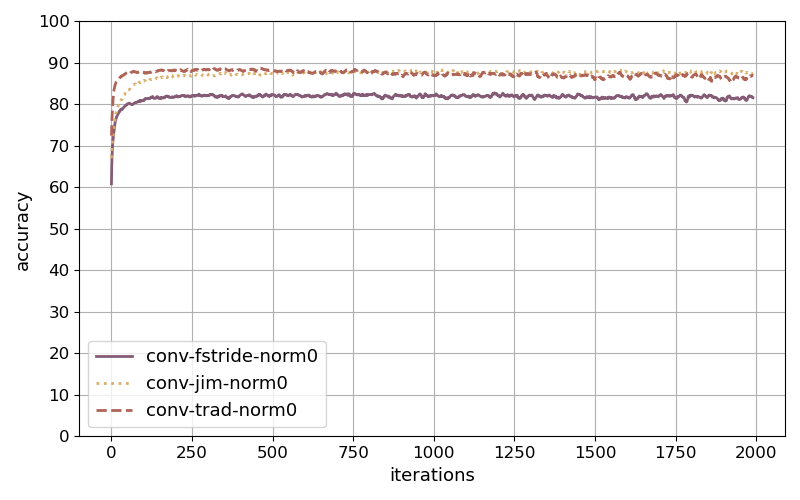
\includegraphics[width=0.45\textwidth]{./5_exp/figs/exp_final_acc_norm0}}
  \subfigure[norm1]{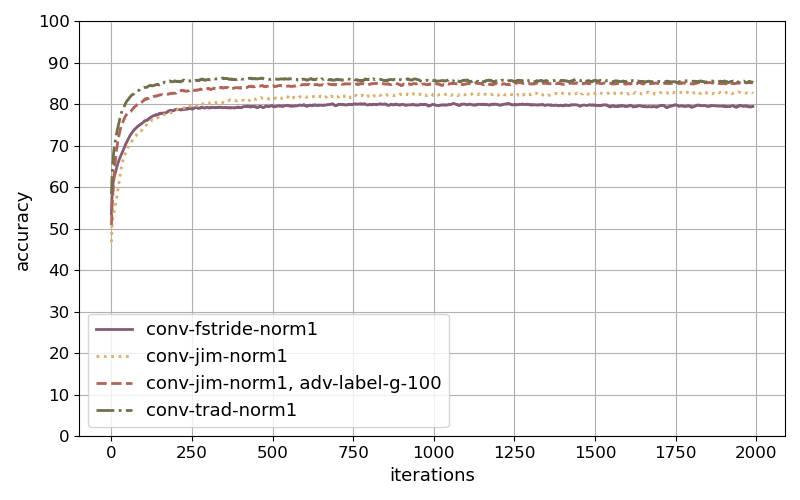
\includegraphics[width=0.45\textwidth]{./5_exp/figs/exp_final_acc_norm1}}
  \caption{Training accuracies of all models with and without frame-based normalization performed on the whole dataset, averaged over 10 epochs for better visualization.}
  \label{fig:exp_final_acc}
\end{figure}
\FloatBarrier
\noindent
Note that the the accuracy score over the epochs are not that smooth and as mentioned before it is strongly recommended to use early-stopping.
That is why the \texttt{conv-trad} without frame-based normalization got a worse score than it would have achieved with early-stopping.